\documentclass[12 pt]{report}
\usepackage[margin=1in, paperwidth=8.3in, paperheight=11.7in]{geometry}
\usepackage[colorlinks]{hyperref}

%\usepackage{graphicx}
\usepackage[final]{graphicx}
\usepackage{subcaption}
\usepackage[utf8]{inputenc}
\usepackage[export]{adjustbox}

\usepackage{listings}
\usepackage{color}

\definecolor{dkgreen}{rgb}{0,0.6,0}
\definecolor{gray}{rgb}{0.5,0.5,0.5}
\definecolor{mauve}{rgb}{0.58,0,0.82}

\lstset{frame=tb,
  language=PHP,
  aboveskip=3mm,
  belowskip=3mm,
  showstringspaces=false,
  columns=flexible,
  basicstyle={\small\ttfamily},
  numbers=none,
  numberstyle=\tiny\color{gray},
  keywordstyle=\color{blue},
  commentstyle=\color{dkgreen},
  stringstyle=\color{mauve},
  breaklines=true,
  breakatwhitespace=true,
  tabsize=3
}


%Table-related commands
\usepackage{array}
\usepackage[table]{xcolor}
\setlength{\arrayrulewidth}{1mm}
\setlength{\tabcolsep}{18pt}
\renewcommand{\arraystretch}{1.5}
\newcolumntype{s}{>{\columncolor[HTML]{AAACED}} p{3cm}}
%-------------------------------------------------------

\usepackage{pgf}
\usepackage{pgfpages}
\usepackage{ragged2e}
\bibliographystyle{plain}
\pgfpagesdeclarelayout{boxed}
{
  \edef\pgfpageoptionborder{0pt}
}
{
  \pgfpagesphysicalpageoptions
  {
    logical pages=1,
  }
  \pgfpageslogicalpageoptions{1}
  {
    border code=\pgfsetlinewidth{3pt}\pgfstroke,
    border shrink=\pgfpageoptionborder,
    resized width=0.9\pgfphysicalwidth,
    resized height=0.9\pgfphysicalheight,
    center=\pgfpoint{0.5\pgfphysicalwidth}{.5\pgfphysicalheight}
  }
}
\pgfpagesuselayout{boxed}

\usepackage{graphicx}

\usepackage{hyperref}
\hypersetup{
    colorlinks=true, 
    linktoc=all,     
    linkcolor=black, 
    citecolor=black,
}
\begin{document}

\begin{center}

\includegraphics[width=6.3in]{images/BVB.png} 
\end{center}



\begin{center}
\begin{Large}
\textbf{\linebreak School of \linebreak \\Electronics and Communication Engineering
}
\end{Large}
\end{center}

\begin{center}
\begin{Large}
\textbf{\linebreak \linebreak Minor Project Report
\linebreak \\on}
\end{Large}
\end{center}

\begin{center}
\begin{LARGE}
\textbf{NON-INVASIVE SMART ENERGY MONITORING SYSTEM}
\linebreak\\
\end{LARGE}
\end{center}

\vspace{2cm}

\begin{flushleft}
\textbf{By:}
\begin{large}
\begin{enumerate}
    \item  \textbf{Shridatha Hegde                  \hspace{5cm}         USN: 01FE18BEC171 }
    \item \textbf{Akhilesh Kumbhar  \hspace{4.5cm}  USN: 01FE18BEC016}
         \item \textbf{Sagar Patil                              \hspace{6.4cm}      USN: 01FE18BEC145}
     \item \textbf{Sai Preetham M                \hspace{5cm}     USN: 01FE18BEC146}
     \item \textbf{Saiprasanna Kuragodi   \hspace{3.6cm}     USN: 01FE18BEC147}

     
\end{enumerate}
\vspace{1cm}
\end{large}

\begin{large}
\textbf{Semester : VI, 2020-2021}
\end{large}
\end{flushleft}

\begin{flushright}
\end{flushright}

\begin{center}

\includegraphics[width=1.5in]{images/certkle.png} 
\end{center}
\begin{center}
\begin{Large}
{\color {violet} \textbf{CERTIFICATE}} \linebreak
\end{Large}
\end{center}


\justify
{This is to certify that project entitled  {\textbf{"Non-Invasive Smart Energy  Monitoring System"}} is a bonafide work carried out by the student team of   \textbf{Shridatha Hegde}        (01FE18BEC171),
\textbf{Akhilesh Kumbhar}    (01FE18BEC016),
\textbf{Sagar Patil}  (01FE18BEC145), \textbf{Sai Preetham M}             (01FE18BEC146), and  \textbf{Saiprasana Kuragodi}    (01FE18BEC147).} The project has been approved as it satisfies the requirements concerning the minor project work
prescribed by the university curriculum for BE (VI semester) in the School of Electronics and
Communication Engineering of KLE Technological University for the academic year 2020-2021.


\vspace{2cm}
\begin{small} \textbf{Dr. Sunita V.B.
}\hspace{2cm} \textbf {   Dr. Nalini C. Iyer } \hspace{2cm} {\textbf{Dr. N.H. Ayachit}} \linebreak
\end{small} 
\vspace{1cm} 
%\begin{large}
\hspace{1.5cm} \small{\textbf{Guide} \hspace{3.6cm}   \textbf{Head of School} \hspace{3.6cm}  \textbf{Registrar}}
%\end{large}


\vspace{0.8cm} 

\begin{flushleft}
\textbf{External Viva: \\}
\end{flushleft}
\textbf{Name of Examiners} \hspace{8cm} \textbf{Signature with date}
\begin{enumerate}
\item  
\item  
\end{enumerate}

\newpage
\begin{center} 
\begin{Large}  
\textbf{ACKNOWLEDGMENT} 
\end{Large}
\end{center}



The satisfactory completion of the project would be incomplete without the mention of many individuals whose professional guidance and encouragement helped us in the successful completion of our work.
We take this opportunity to express a deep sense of gratitude to Dr. Ashok Shettar, Vice-Chancellor, KLE Technological University, and Dr.Nalini C. Iyer, Head of the department, School of Electronics and Communication Engineering for providing the necessary facilities required for completion of this project and their exemplary guidance, monitoring and constant encouragement throughout the course of this project.
\par We would also like to express our sincere gratitude towards our project guides Dr. Sunita V.B. and Dr. Saroja V.S.  whose constant guidance and care made the project successful.




\flushright
- The Project Team


\flushleft


\newpage
\begin{center}
\begin{Large}
\textbf{ABSTRACT}

\end{Large}
\end{center}
\justifying
Smart home devices and its applications have a great upside potential in successfully cutting down the electricity consumption across households. This study focuses on the realisation of the potential that the application provides. As an initial process, the current consumption is measured and stored in a database with the help of PHP via the ESP 32 microcontroller. The AWS cloud services is used for the users to view consumption in real-time. Data acquired  is utilised by the server to run LSTM Neural Networks to predict the possible future usage. This predicted future value is compared with the actual consumption to test the accuracy of the model.



\newpage
\tableofcontents



\listoffigures


\newpage
\chapter{Introduction}
The electricity bill generated by the electricity supply company can be often confusing as it does not explain the consumption of individual rooms or labs or cabins but instead, the bill provides a sum of all these as a whole. So this project as a whole tries to explain the power consumed individually by these sections. Predicting the possible power consumption is a very important job at hand as this helps to plan the consumption accordingly. Using different machine learning algorithms, these possible future values would be sought.

\section{Objectives}
\item The objective of the project includes

\begin{itemize}
\item To design and develop a data acquisition system for measuring energy consumption
\newline

\item To Visualize and forecast consumption usage with cloud computing
\newline

\item To make energy monitoring smarter
\newline
\end{itemize}

\section{Problem Statement}
To design and develop a non-invasive smart energy monitoring system.

 \newpage 
\section{Literature Survey }


\begin{itemize}
\item \underline{Paper 1} described about a novel experimental prototype IoT system which demonstrates the real time location-based automated energy policy control across multiple buildings. It is the basic step in changing from the current centralized control and static energy consumption modes to distributed and dynamic energy control in the consumer-side smart grids containing various common buildings. The modeling and evaluation results are used to identify the key energy components of the building, to apply adjustments, and to devise strategies to reduce energy consumption. IoT based networking system is designed and prototyped to realize the strategies and achieve the goal.
\newline
\end{itemize}

 \begin{itemize}
\item \underline{Paper 2} aimed to answer the question of how to incorporate Big Data platform and machine learning into an intelligent system for managing energy efficiency of public sector as a substantial part of the smart city concept. Deep neural networks, Rpart regression tree and Random forest with variable reduction procedures were used to create prediction models. The paper also discusses technological requirements for developing such a platform that could be used by public administration to plan reconstruction measures of public buildings, to reduce energy consumption and cost, as well as to connect such smart public buildings as part of smart cities.
\newline
\end{itemize}


  \begin{itemize}
\item \underline{Paper 3}, a brief introduction on smart homes was learned. A smart home represents also a home that satisfies its needs in an intelligent and flexible ways, responding to the needs and comfort of its dwellers, enabling them to control and manage consumption of their own green energy sources. The aim of this article is to present a cost effective energy management system design and implementation suitable for frugal smart cities. The paper focuses on proposing a solution of continuous monitoring system constituted by connected energy metering and control devices based on Arduino and Raspberry Pi and remotely controlled, via WiFi, current and voltage smart meters/switches. This cost effective monitoring system was wirelessly connected to an application installed in a computer mobile device, to collect energy production/consumption data and operate control actions.
\end{itemize}

\section{Organization of the Report}
The report is divided into 4 parts. Each part (chapter) deals with different aspects of the project.\newline
1) Chapter 1 discusses about the motivation behind the project, main objectives, formation of the problem statement and the literature survey done by the team.\newline 
2) Chapter 2 discusses about the proposed methodology and its implementation.
\newline 
3) Chapter 3 discusses about the results achieved of the proposed methodology and Optimization used to get the result.\newline 
4) Chapter 4 provides the conclusion and briefs on the future scope of the project.\newline
The Appendix Section states all the references used in the project.


\newpage
\chapter{Proposed Methodology}
 In this chapter, we discuss about our proposed design, which includes steps for setting up various tools required for the proper functioning of the system. This chapter also gives an insight about the system framework used in this project.
 
 \section{System design}
 \item 

Systems design is the process of defining the architecture, product design, modules, interfaces, and data for a system to satisfy specified requirements. We shall discuss the proposed system framework for the problem statement.
\subsection{Proposed Functional block diagram of system}
\begin{figure}[h!]
\centering
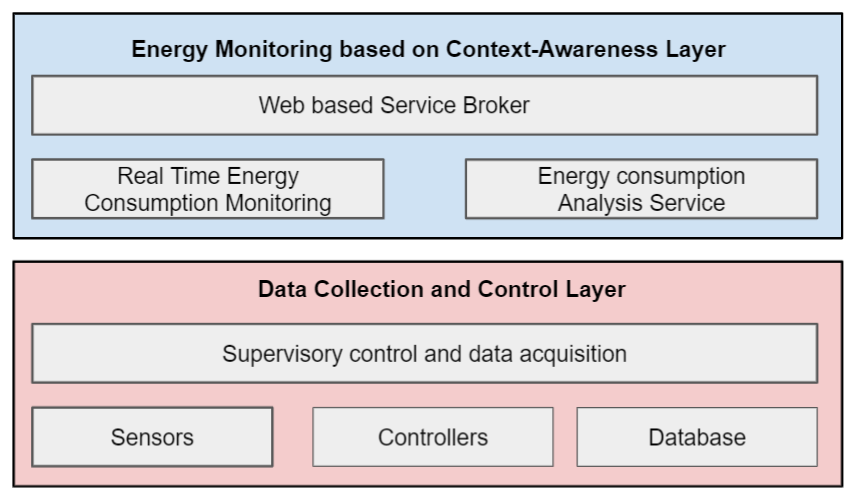
\includegraphics[width=16cm,height = 10cm,frame]{images/problock.png}
\caption{The proposed energy monitoring block diagram with first layer based on context awareness and second layer as data collection control.}
\label{fig:Proposed Block Diagram of system}
\end{figure}
The framework consists of two layers and performs various functions including those of the above figure. First, the data collection and control layer consists of non-invasive current sensors and an ESP32 controller. The Sensors collect the current usage (in Amp) and the controller performs energy consumption data calculation (in KWh). The data is stored in a cloud service database.The database has the tables for the raw data and converted data from the sensors. The energy management based on context-awareness layer administrates databases (DBs), with a front-end web interface for real-time data visualization for the user. Also with the employment of deep learning neural network-based model, analyses the past and present energy consumption and predicts future energy consumption. Also, the layer generates the
improved methods of energy management and forecasts the effects and performance indicators.

\subsection{Morphological Chart}
A morphological chart is a tool that represents a large qualitative design space. These charts list the functions identified for the design problem. We have selected the combination of CT sensor, Esp32 and AWS EC2.
 \begin{figure}[h!]
\centering
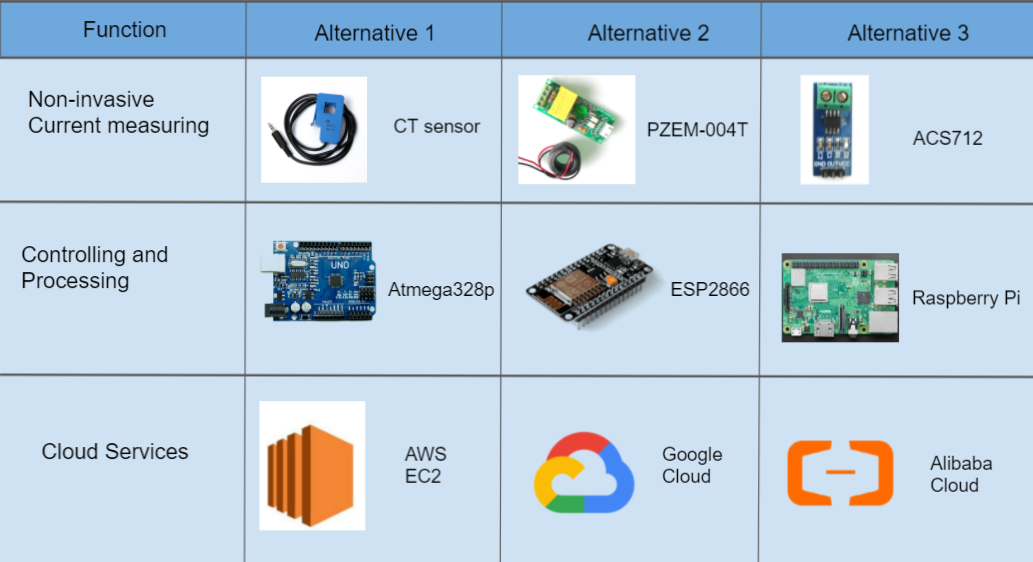
\includegraphics[width=18cm,height = 11cm,frame]{images/morph.png}
\caption{Morphological chart, each function has 3 alternatives}
\label{fig:Morphological chart}
\end{figure}

 \newpage
 
\subsection{System Framework}
 \item The tools used while working on the project have been listed below. The explanation on how each tool used in this project is explained in the next sections.
 \newline
 \begin{table}[ht]
     \centering
   \begin{tabular}{||c| c||}
  \hline
     Tool  &  Usage\\ [0.5ex]
  \hline\hline   
     SCT-013 sensor  &  Electric Current Measurement\\
  \hline   
     ESP32 Devkit V1 Microcontroller  &  Data reception and transmission\\
  \hline 
     Battery Pack, USB supply  &  Power Source\\
  \hline
     Ubuntu  &  AWS Cloud Server\\
  \hline   
     php, html, javascript  &  Data Visualization\\
  \hline
     mySQL  &  Data Storage\\
  \hline 
     python  &  Machine Learning Model\\
  \hline 
     flask  &  Web Application Deployment\\ [1ex]
  \hline 
  \end{tabular}
  \caption{Proposed System Framework}
   \end{table}




%%%%%%%%%%%%%%%%%%%%%%%%%%%%%%%%%%%%%%%%%%%%%%%%%%%%%%%%%%%%%%%%%%%%%%%%%%%%%%%%
\section{Data Acquisition Implementation}

It  implies how the data is being  collected from the sensor node and how the collected data is transmitted to the database.
\subsection{Setting up sensor node}

\begin{figure}[ht]
\begin{subfigure}{.5\textwidth}
  \centering
  % include first image
  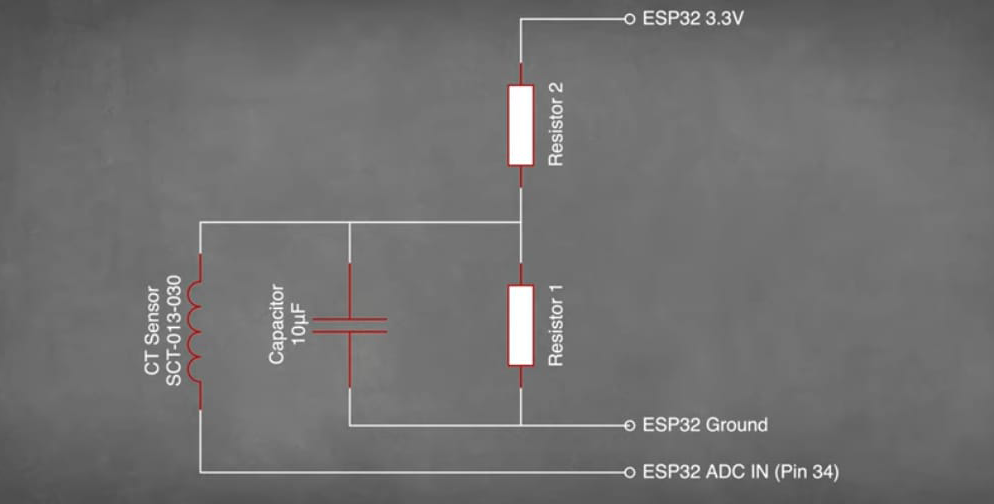
\includegraphics[width=1.05\linewidth,frame]{images/circuit.png}  
  \caption{Circuit Diagram}
  \label{fig:Circuit Diagram}
\end{subfigure}
\begin{subfigure}{.5\textwidth}
  \centering
  % include second image
  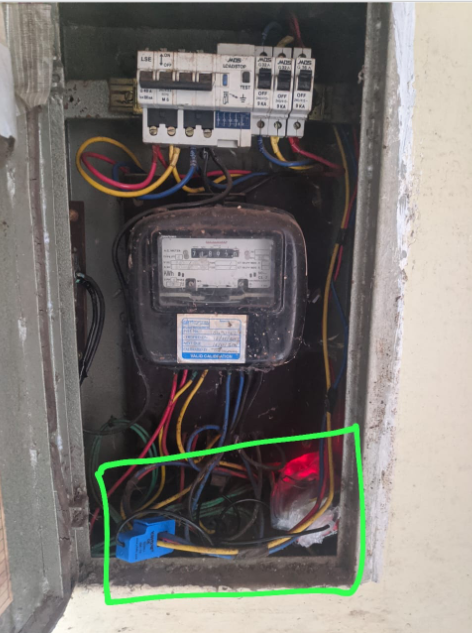
\includegraphics[width=.7\linewidth]{images/setup.png}  
  \caption{Sensor setup}
  \label{fig:Sensor setup}
\end{subfigure}
\caption{Sensor node}
\label{fig:Sensor node}
\end{figure}
A non-invasive current transformer sensor is used to calculate the amount of current flowing through a live wire from mains using the concept of, Hall effect. The sensor is a capable of reading the current values up-to 30A. Due to technology, the sensor may produce output voltage when no current is flown through sensor. System need to know this offset in order to properly calculate actual current flow. Two resistors of the same within the range of 100 ohms to 470k ohm are used to generate a voltage divider circuit which acts as calibration setup.

\subsection{Data acquisition and storage}
  \begin{figure}[h!]
\centering
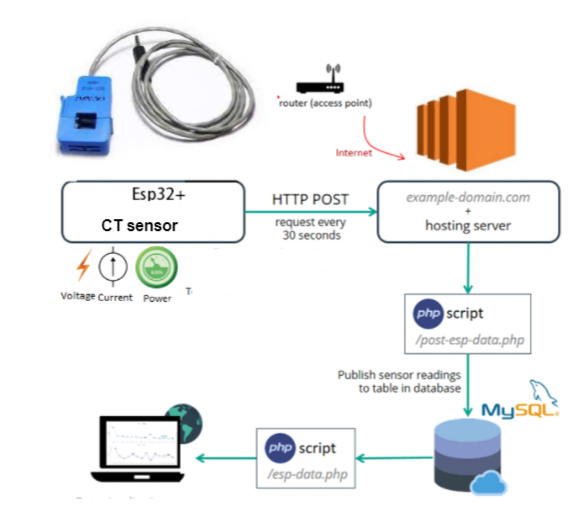
\includegraphics[width=10.7cm,height = 8cm,frame]{images/flow.png}
\caption{Data acquisition system with server as infrastructure}
\label{fig:Data acquisition system with server as infrastructure}
\end{figure}


 

 Data acquisition is the process of taking samples of signals that measure real-world physical parameters and transforming them into digital numeric values that a computer can alter.
 \newline
 In this project, we build an ESP32  client that makes an HTTP POST request to a PHP script to insert data (sensor readings) into a MySQL database.
 \newpage
\underline{The procedure follows as- }
 \newline
  \newline
 \textbf{1.Setting up  ESP32}
 \newline
 \newline
a. Flashing the ESP32 with a  new API key and WIFI credentials.
 \newline
b. Connect the sensor to the respective analog pin and clamp sensor either to live or neutral wire.


\newpage

 \textbf{2.Hosting PHP Application and MySQL Database}
   \begin{figure}[h!]
\centering
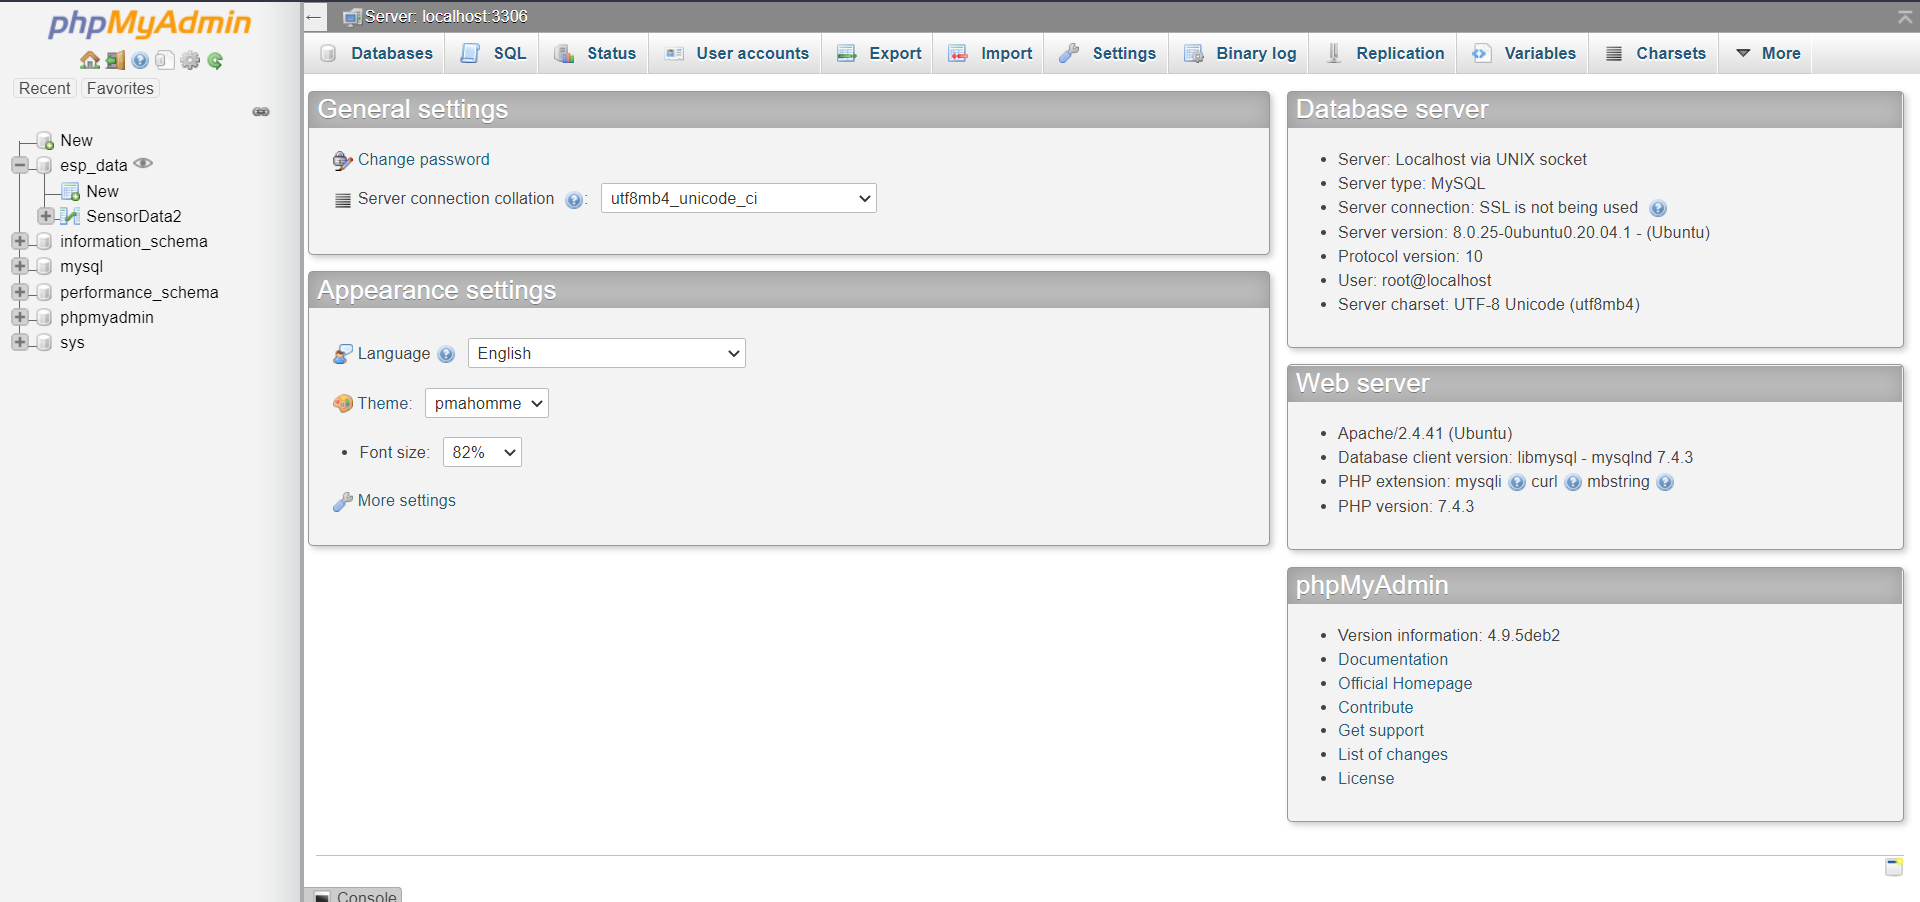
\includegraphics[width=12cm,height = 7cm]{images/phphome.png}
\caption{MySQL database installed with the phpmyadmin and Linux Apache server to connect to the database}
\label{fig:MySQL database}
\end{figure}
\newline

 \textbf{3.Creating SQL table}
 \newline
 
 
 \begin{table}[]
\centering
 \begin{tabular}{||c| c ||} 
 \hline
 Table Attributes & Data type \\ [0.5ex] 
 \hline\hline
 id (Primary Key) & integer \\ 
 \hline
 value1 & varchar \\
 \hline
 value2 & varchar \\
 \hline
 readingtime & timestamp \\ [1ex] 
 \hline
\end{tabular}
\caption{SQL table structure}
 \end{table}
 
 The id is used as a serial number which increments by itself and acts as primary key for the table. The values from sensor1 and sensor 2 are stored in value1 and value2 column respectively. The reading time will record thet time at which data was logged.
   
 \begin{figure}[h!]
\centering
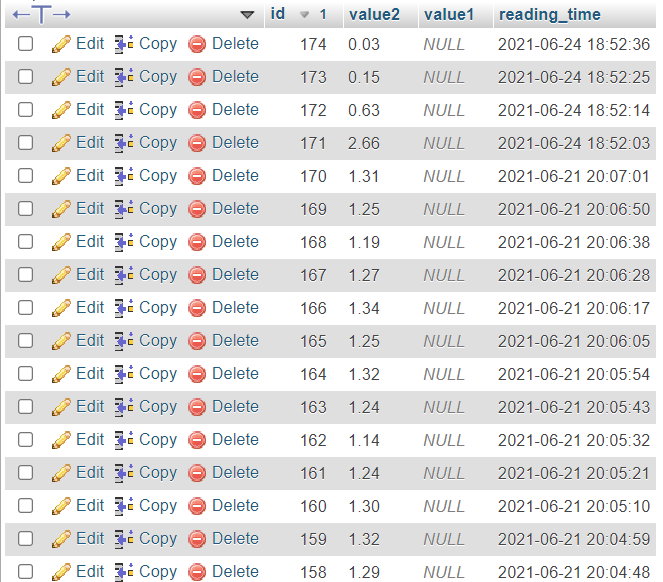
\includegraphics[width=10cm,height = 7cm,frame]{images/table.png}
\caption{Table attributes}
\label{fig:Table attributes}
\end{figure}
\newpage

 \textbf{4.Insert Data in MySQL Database, using PHP Script HTTP POST}
 \newline
 1) connect to database with credentials.
 \newline
 2) create unique API key value.
 \newline
 3)assign api key value to table.
 \newline
 4) whenever http post is requested store the value in respective column.
 \newline

\section{Data Analysis and Forecasting}
\subsection{Data Pre-processing}
The reference dataset from Kaggle contains measurements of electric power consumption in one household with a one-minute sampling rate over a period of almost 4 years.
\newline
Attribute Information:
\newline
1.date: Date in format dd/mm/yyyy

2.time: time in format hh:mm:ss

3.globalactivepower: household global minute-averaged active power (in KW)

4.globalreactivepower: household global minute-averaged reactive power (in KW)

5.voltage: minute-averaged voltage (in V)

6.globalintensity: household global minute-averaged current intensity (in A)

7.totalconsumption: Combined household consumption from three sub-meterings (in KWh)
\newline

 The dataset was resampled from minute to hourly frequency for better pattern analysis and seasonal trends. The columns of features 'globalactivepower','totalconsumption' along with time were considered for the prediction model.
  \begin{figure}[h!]
\centering
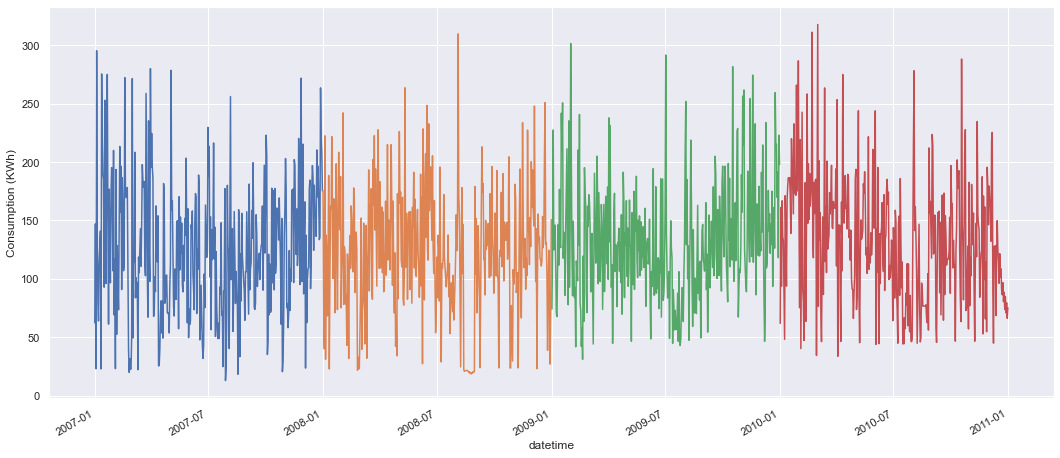
\includegraphics[width=16cm,height = 8.5cm,frame]{images/eda1.png}
\caption{Overview of dataset visualization with selected feature as consumption (in kWh) and timestamp set as index.}
\label{fig:Dataset Overview}
\end{figure}

\newpage 
\subsection{Exploratory Data Analysis}

The exploratory analysis helps to identify obvious errors, as well as better understand patterns within the data, detect outliers or anomalous events, find interesting relations among the variables.  
\newline
  
  To check whether the data used was stationary or not, Augmented Dickey Fuller Test was conducted on the data. The test results further proved that data is indeed stationary as the 'p-value' obtained (0.000483) was less than 0.05 and hence it rejects the Null Hypothesis, data has no unit root and is stationary.
    \begin{figure}[h!]
  \centering
  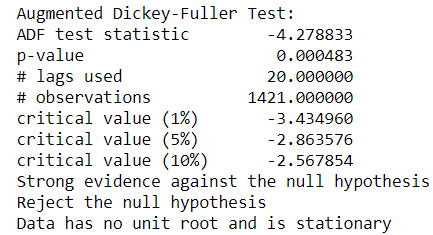
\includegraphics[width=12cm,height = 7cm,frame]{images/ADF.png}
  \caption{Stationarity Check using Augmented Dickey Fuller Test shows that 'p-value' obtained (0.000483) was less than 0.05 and hence it rejects the Null Hypothesis, data has no unit root and is stationary.}
  \label{fig:Stationarity Check using Augmented Dickey Fuller Test}
  \end{figure}
  
    
    \begin{figure}[h!]
  \centering
  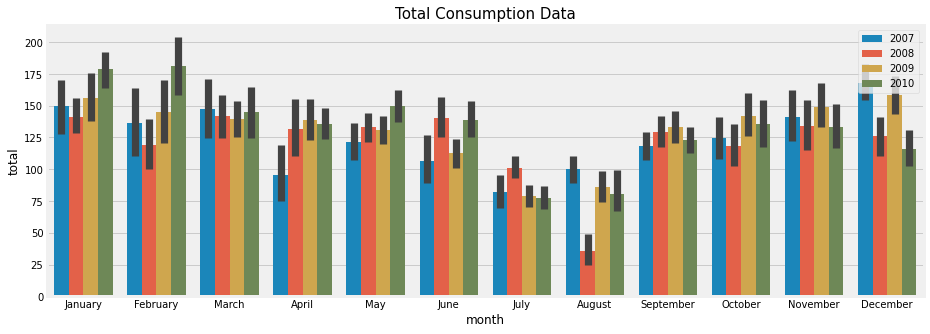
\includegraphics[width=14cm,height = 8cm,frame]{images/eda2.png}
  \caption{Comparison of electricity consumption month wise during different years depicting increasing trend of usage by years.}
  \label{fig:Monthwise aggregate usage}
  \end{figure}
  
\begin{figure}[h!]
  \centering
  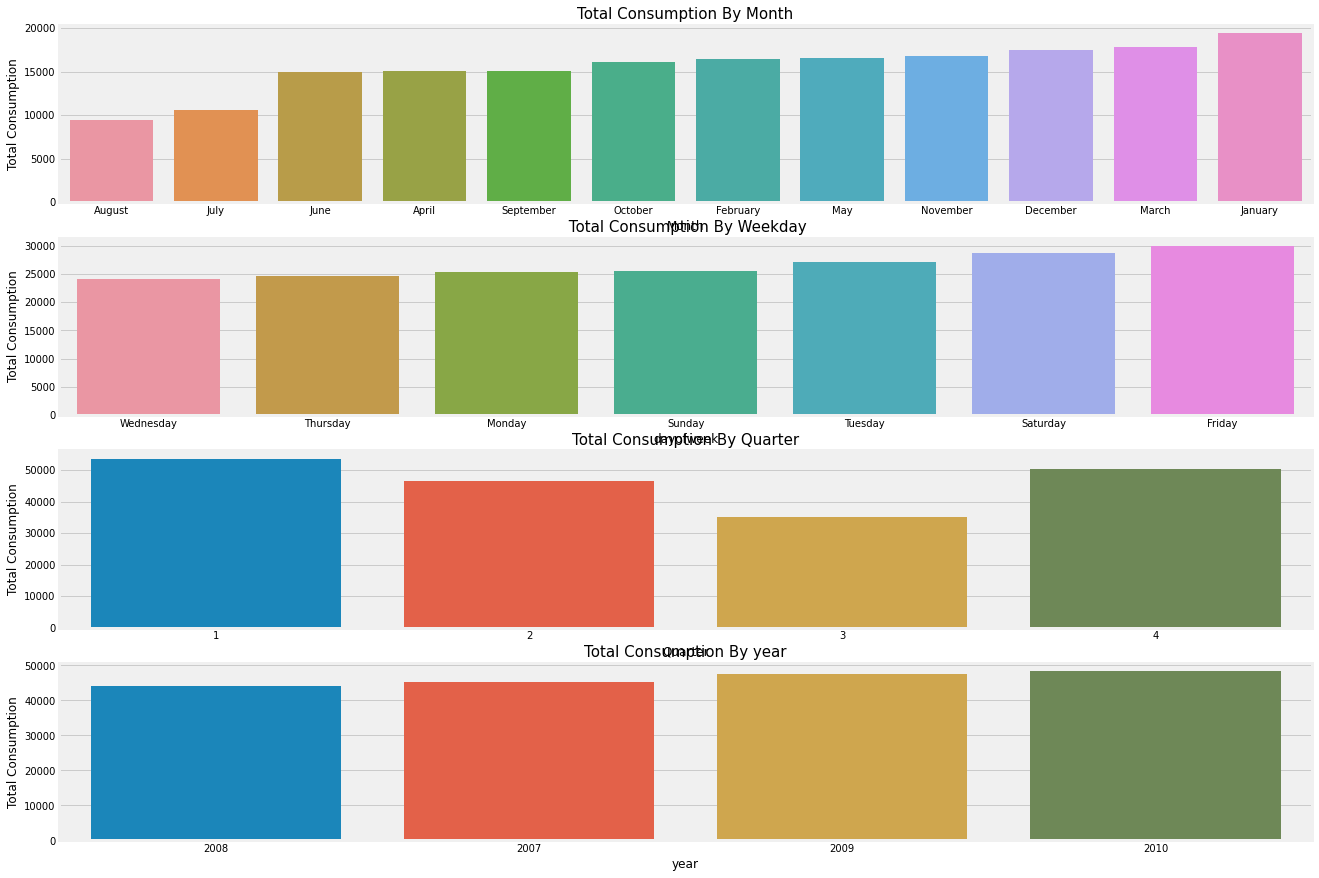
\includegraphics[width=12cm,height = 8cm,frame]{images/eda3.png}
  \caption{exploded view of dataset with consumption analysis by every weekday, month,quarter and year depicting seasonality.}
  \label{fig:Usage bargraph}
  \end{figure}

\newpage

\subsection{LSTM Neural Networks}

    Long Short Term Memory networks – usually called “LSTMs” – are a special kind of RNN, capable of learning long-term dependencies. RNN's are the state of the algorithm for the sequential data. It remembers the input due to internal memory.
\newline For sequence models, it is found that rather than features, it is more largely dependent on past values which becomes deciding factor for the next day forecast. LSTMs have an edge over conventional feed-forward neural networks because of their property of selectively remembering patterns for a long duration of time.
\newline
\newline
\underline{Architecture}
\newline
The LSTM Architecture consists of four components-
\newline
1. \textbf{Memory Gate}- It is like a conveyor belt that runs straight down the entire chain, with gate interactions. The Gate is a structure that regulates adding/removing information to the LSTM.
\newline
2. \textbf{Forget gate}- It is responsible for removing information from the cell state. The information which is no longer required for the LSTM to understand the  things are removed. This optimizes the performance of the network.
\newline
3. \textbf{Input gate}- It is responsible for the addition of information to the cell state. This ensures that only that information is added to the cell that is important and not redundant.
\newline
4. \textbf{Output gate}- The job of selecting the useful information from the current cell state and showing it out as output is done by this gate.
\newline


\begin{figure}[ht]
\begin{subfigure}{.5\textwidth}
  \centering
  % include first image
  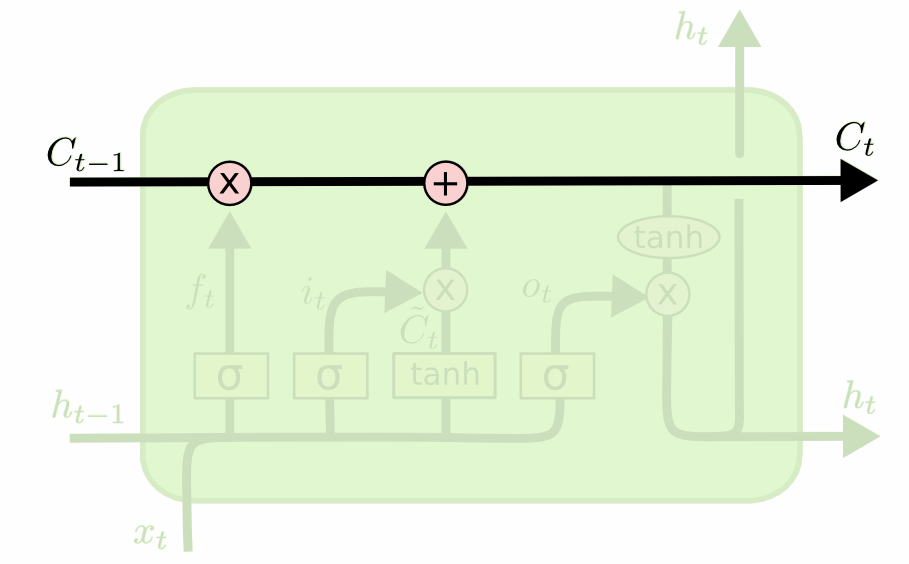
\includegraphics[width=.8\linewidth,frame]{images/memgate.png}  
  \caption{Memory Gate}
  \label{fig:Memory Gate}
  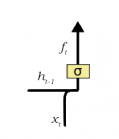
\includegraphics[width=.6\linewidth,frame]{images/forgate.png}  
  \caption{Forget Gate}
  \label{fig:Forget Gate}

\end{subfigure}
\begin{subfigure}{.5\textwidth}
  \centering
  % include second image
      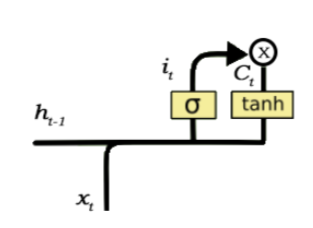
\includegraphics[width=.8\linewidth,frame]{images/ingate.png}  
  \caption{Input Gate}
  \label{fig:Input Gate}
  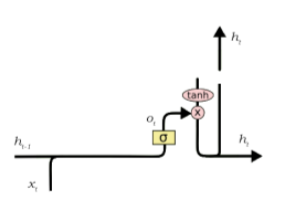
\includegraphics[width=.8\linewidth,frame]{images/outgate.png}  
  \caption{Output Gate}
  \label{fig:Output Gate}
\end{subfigure}
\caption{LSTM Architecture}
\label{fig:fig}
\end{figure}

 \newpage
\underline{Implementation with Tensorflow}-
\newline
\newline
  The daily resampled dataset contains 1460 samples. 80 percent of this data is split into train and the remaining 20 percent as test data to validate the accuracy of the model. The train and test data were normalized using MinMax Scaler which converts the entire data into the range of (0,1). The scaled data is converted into a NumpPy array. 
  The TensorFlow takes input in the form of 3D tensors. Hence the data is reshaped by creating batches of the dataset. We specify the batch size as the parameter to consider for our future prediction along with timesteps. 
  \newline
  The sequential model is imported and two hidden layers of LSTM are added with each layer having 60 input neurons. A dropout layer is added which helps to deactivate the layers whose output is zero. A dense layer with "relu" activation function is included which acts as the output layer of the model.
  
\begin{figure}[h!]
  \centering
  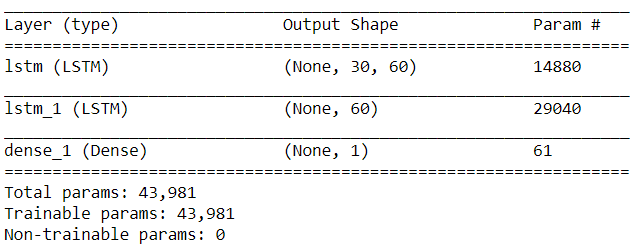
\includegraphics[width=16cm,height = 8cm,frame]{images/modelsummary.png}
  \caption{LSTM Model summary}
  \label{fig:LSTM Model summary}
  \end{figure}

\newpage 

\section{Cloud Services}
\par 

\subsection{Saving weights as model file}
    As discussed in the previous chapter,the LSTM architecture is used to train the model. The model is saved as a h5 file so that it can save the program’s state data to disk and carry on where it left off when restarted. It is a structured format to save model's weights and configuration in a single file.
\newline

\subsection{AWS EC2 instance}
An EC2 instance is a virtual server in Amazon’s Elastic Compute Cloud (EC2) for running applications on the Amazon Web Services (AWS) infrastructure. EC2 is a service that allows users to run application programs in the computing environment AMI is a template that contains the software configuration (operating system, application server, and applications) required to launch the instance. It is a Ubuntu 20.04, Linux-based OS. A public DNS will be generated which would be used in the next steps. We create new security with network traffic set to ALL and accessible for anyone from anywhere and link this to our instance through network interfaces and permissions.

 \subsection{SSH Client}
    After creating and launching an EC2 instance, to access it an SSH client is needed. With the help of public DNS of instance and username along with private key one can access remotely with SSH client.
    \par
    We use Putty SSH client which is a free open source serial console and network application for connecting and working with the command line interface of the Ubuntu server.
    
    \begin{figure}[h!]
     \centering
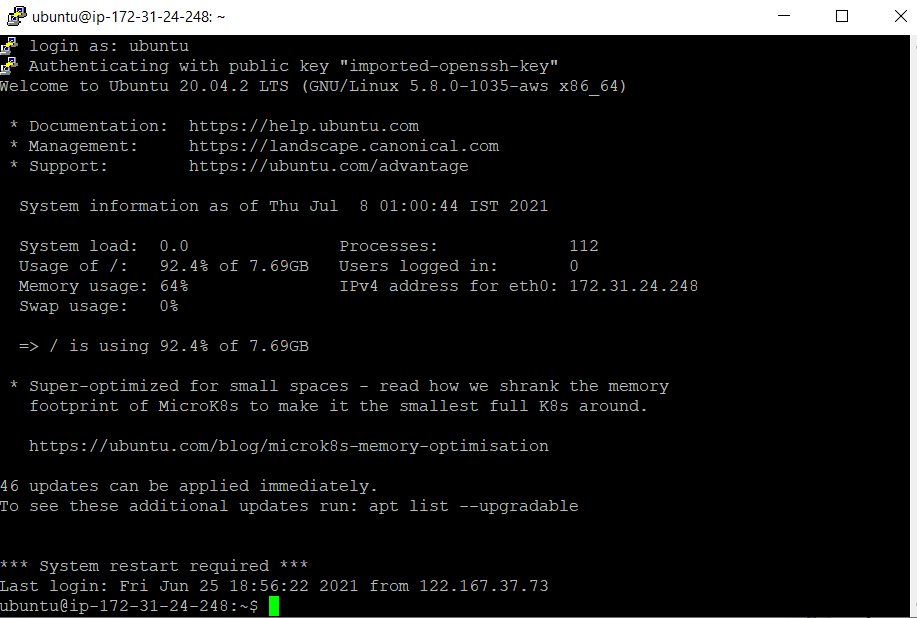
\includegraphics[width=12cm,height =8cm,frame]{images/putty.png}
\caption{ Putty SSH Client}
\label{fig:Connecting to server via SSH client}
\end{figure}
\newpage
  
  \subsection{Secure Copy Protocol}

 WinSCP is a free and open-source SFTP, FTP, Amazon S3, and SCP client for Microsoft Windows. Secure copy protocol (SCP) is a means of securely transferring computer files between a local host and a remote host or between two remote hosts. \par It is based on the Secure Shell (SSH) protocol.  
We use the private key with WinSCP to copy all our model files into the server.
\begin{figure}[h!]
 \centering
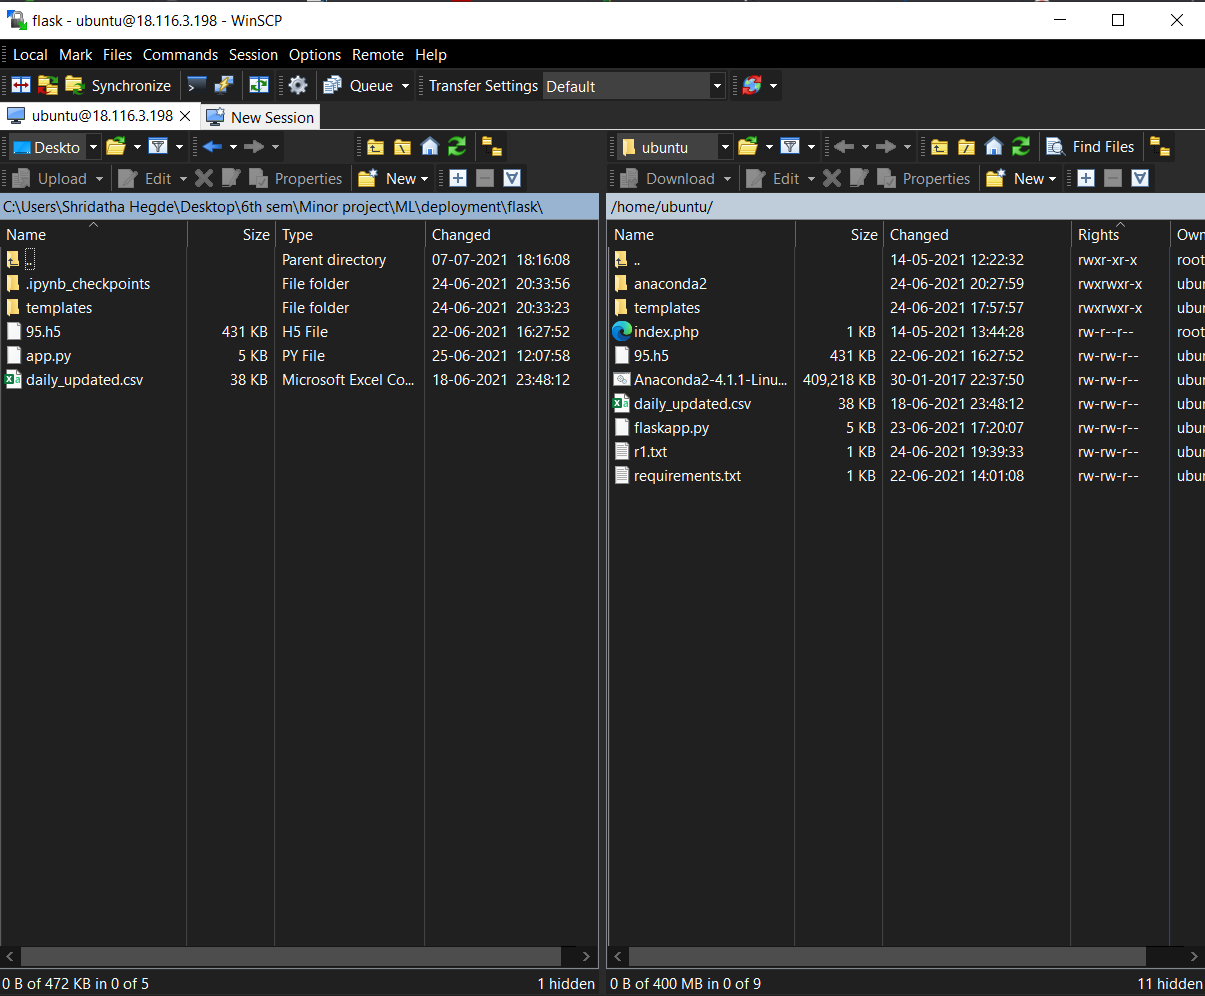
\includegraphics[width=12cm,height = 8cm,frame]{images/scp.png}
\caption{ Transferring files into Server}
\label{fig:Transferring files into Server}
\end{figure}


\subsection{Real-time Visualization}
The frontend for the real time graphs is done with php,html, javascript with MySQL acting as backend which provides data from it's table.
\begin{itemize}
    \item Access database through php script
    \item Check and verify connection with database
    \item Create chart using HTML5  based JavaScript to generate interactive graphs on html web pages.
\end{itemize}



 \section{User Interface}
 UI is the top layer at which human users can interact with the application. Here we have developed a Web based graphical user interface to visualise electricity consumption in real time and forecast based on the past consumed units.\par
Flask Web framework is an API of Python that allows us to build up web-applications. Flask is based on WSGI(Web Server Gateway Interface) toolkit and Jinja2 template engine.  Flask does not include a database abstraction layer. We use this to create a web-API that would display the prediction in an HTML page using POST method request which means the model will take input from the user through HTML and returns the predicted value. By defining the app route the HTML page is rendered.
  
% { Web API}
  \begin{figure}[h!]
\centering
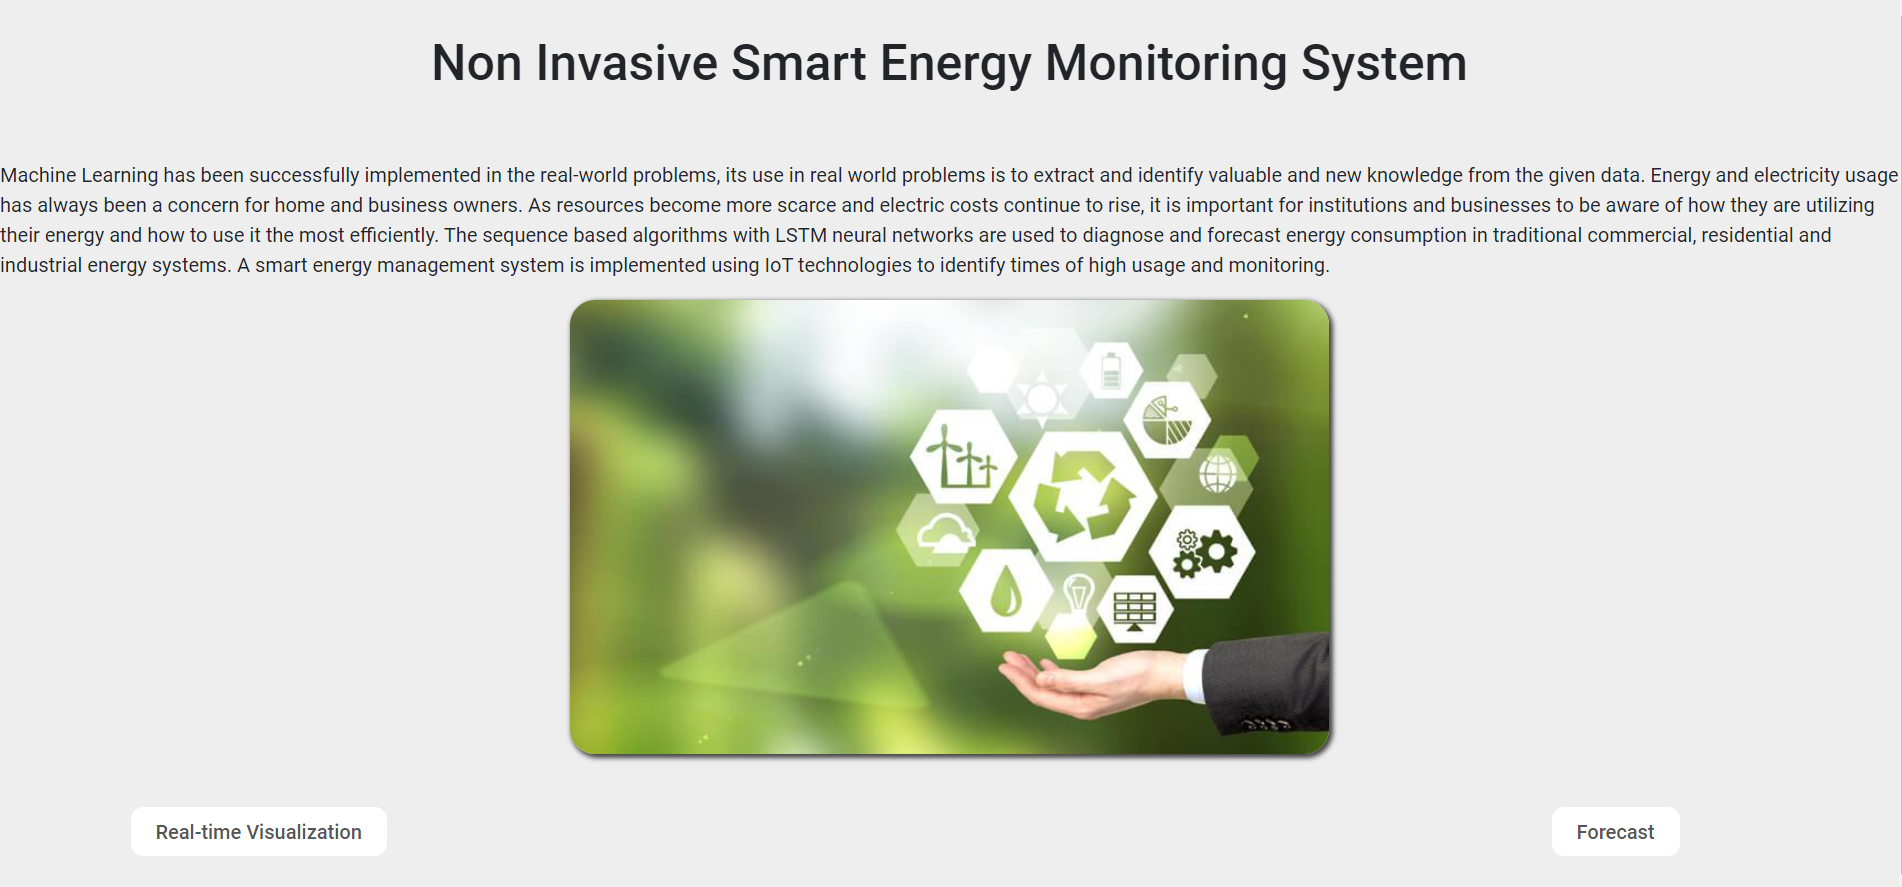
\includegraphics[width=16cm,height = 8cm,frame]{images/homepage.png}
\caption{An interactive based graphical interface  acting as homepage.}
\label{fig:homepage of energy monitoring system}
\end{figure}

 \begin{figure}[h!]
 \centering
 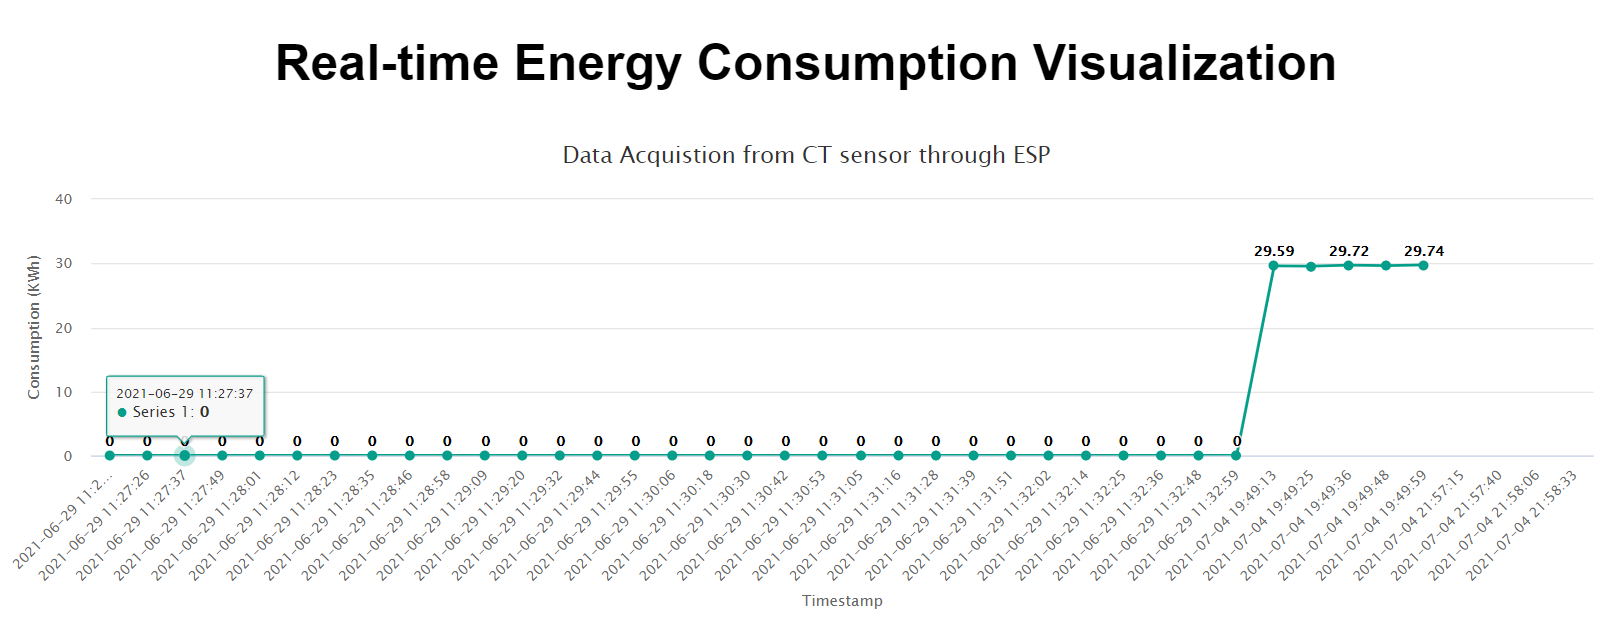
\includegraphics[width=16cm,height =8cm,frame]{images/dashboard.png}
 \caption{Dashboard for real-time visualization made with creative chart which displays data acquired from sensor (consumption value in kWh).}
 \label{fig:Dashboard depicting Realtime usage}
\end{figure}

\begin{figure}[h!]
 \centering
 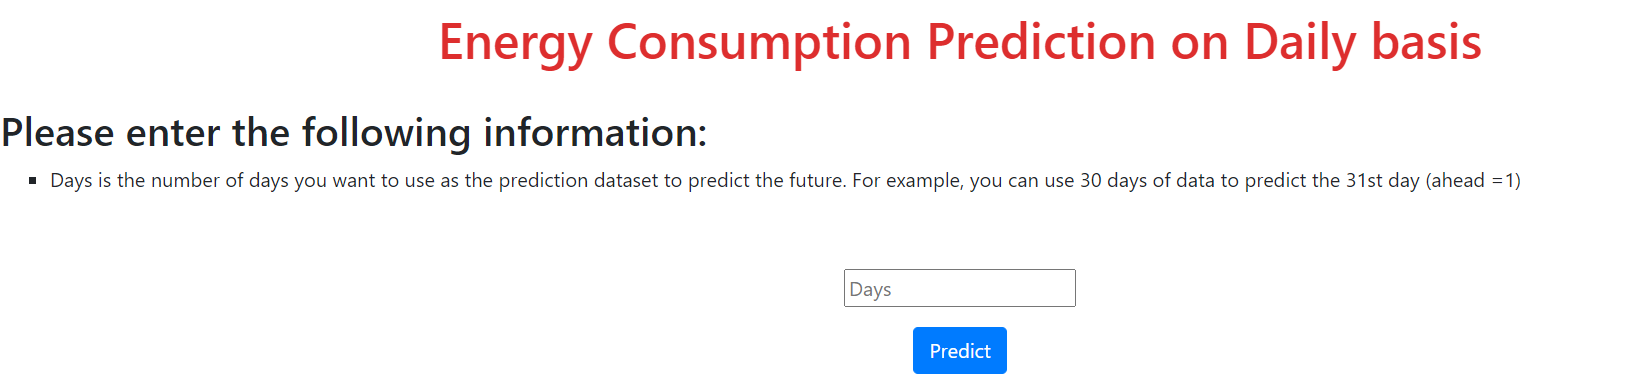
\includegraphics[width=17cm,height = 4.5cm,frame]{images/form.png}
 \caption{GET request based html webpage for taking number of days to be used as input to predict the future for the LSTM model.}
 \label{fig: Form for user input}
\end{figure}

\begin{figure}[h!]
 \centering
 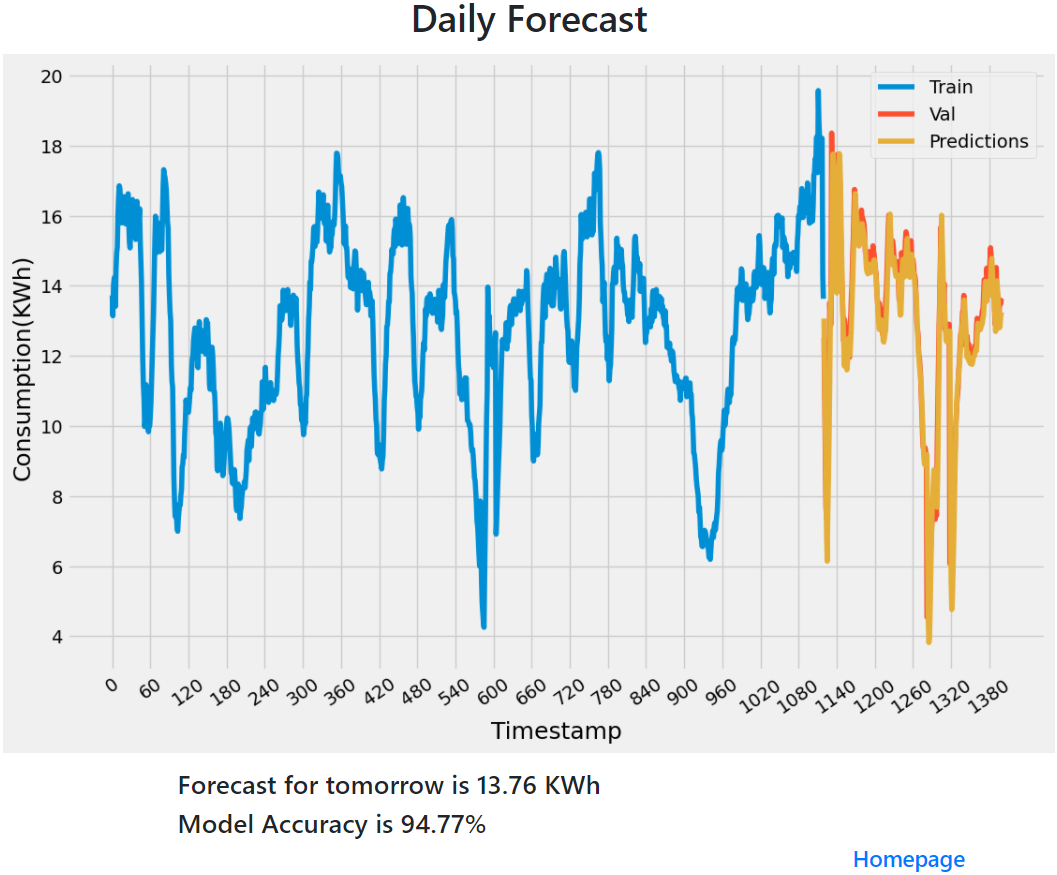
\includegraphics[width=17cm,height = 11cm,frame]{images/results.png}
 \caption{Plot of forecast model with train, validation and predicted data values rendered from LSTM model through flask API, along with forecast for the next timestamp (next day) and model accuracy.}
 \label{fig:Forecast Results}
\end{figure}


\newpage

\chapter{Results and discussions}

In this chapter, we discuss about the results achieved, the optimization used to achieve it and analysis of the results.

\section{Optimization}
Optimization is a procedure that is executed iteratively by comparing various solutions till an optimum or a satisfactory solution is found.
\newline
A well optimized system is low power consuming, with an optimum operation coverage, cost effective and compact. All the quoted factors help a system function near perfectly.

\subsection{Hardware optimization}
Efficient use of power is a concern that should not be neglected.ESP32 uses 240mA in active mode ,this small number can be problematic in the long run, thus to control the power consumption 5 configurable power modes can help in power management of the overall system. The different modes are
\newline
1.\textbf{Active Mode}
\newline
2.\textbf{Modem sleep mode}
\newline
3.\textbf{Light sleep mode}
\newline
4.\textbf{Deep sleep mode}
\newline
5.\textbf{Hibernation sleep mode}
\newline
For our setup  convenient  mode is the light sleep mode.In \textbf{Light sleep mode} digital peripherals,CPU and RAM are clock-gated.The CPU is halted by turning off its clock pulses in light sleep mode, although the RTC and ULP-coprocessor remain functioning. This uses less power than the modem's sleep mode, which uses roughly 0.8mA. 

\subsection{Deep learning model optimization}
In this section, we shall discuss improving the accuracy of the model employing hyper parameter tuning.  A hyperparameter is a parameter whose value is used to control the learning process.  Hyperparameter optimization finds a tuple of hyperparameters that yields an optimal model which minimizes a predefined loss function on given independent data.
\newline

List of hyper parameters taken into consideration-
\newline
1.\textbf{ Batch Size}- Number of data feeding in batches for the model
\newline
2.\textbf{Learning Rate}- Parameter used to control how much to change the model in response to the estimated error each time the model weights are updated.
\newline
3.\textbf{Epoch}- The number of passes the entire training dataset the algorithm has completed.

4.\textbf{Optimizer}- Update the various parameters that can reduce the loss in much less effort. Adam optimizer is used as it helps to identify global minima quickly.
\newline
5.\textbf{Loss function}-  It is a method of evaluating how well specific algorithm models the given data. The usage of MAE gradient is large, which can lead to missing minima at the end of training. Huber loss helps to identify and correct this.
\newline

% \newpage

\begin{figure}[h!]
 \centering
 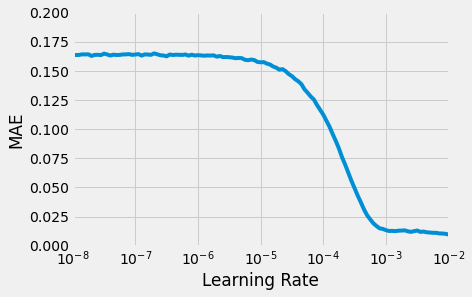
\includegraphics[width=10cm,height = 6cm,frame]{images/figure.png}
 \caption{ learning rate scheduler is used with over 100 epochs, for selecting optimal learning rate and plotted with y-axis as MAE against x-axis as the learning rate.}
 \label{fig: MAE vs Learning Rate}
\end{figure}

\begin{figure}[h!]
 \centering
 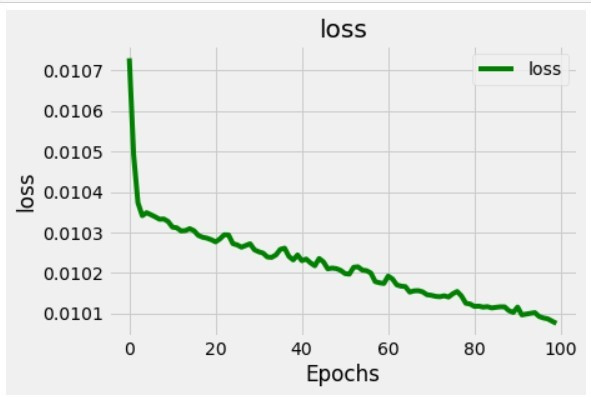
\includegraphics[width=10cm,height =6cm,frame]{images/loss.jpg}
 \caption{the optimal learning rate of 0.002 is used to train the model with 120 epochs to reduce the MAE with much better convergence to deliver improvement in model accuracy.}
 \label{fig:Loss vs Epoch}
\end{figure}

\newpage
\section{Result Analysis}

Literature survey of different papers and publications yielded the decision matrix for selecting the best suited system for proof of concept. Various prediction models including both statistical and machine learning were taken into consideration for appropriate trade off. The usage of the deep learning approach with LSTM architecture resulted in better forecast accuracy of the model.
 \begin{figure}[h!]
\centering
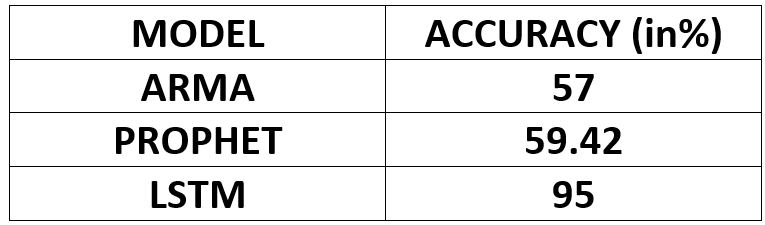
\includegraphics[width=12cm,height = 5.5cm,frame]{images/models.png}
\caption{Model accuracy comparison}
\label{fig:Models accuracy comparison}
\end{figure}
\newline 
% The LSTM model worked well with the dataset, as it gave an accuracy of 80\%. After it's hyper-parameters were tuned, the model achieved an accuracy of 95\%. The below table shows how the hyper-parameters were tuned.

   \begin{tabular}{||c|c||}
  \hline
     Hyperparameters  &  Description/Value\\ [0.5ex]
  \hline\hline   
     Epochs  &  120\\
  \hline   
     Optimizer  &  Stochastic Gradient Descent (SGD) Optimizer\\
  \hline 
     Loss Function  &  Huber Loss Function\\
  \hline
     Metrics  &  Mean Absolute Error (MAE)\\
  \hline   
     Learning Rate  &  0.002\\
  \hline
     Batch Size  &  80\\
  \hline 
     Train Size  &  1120 (80\% of data)\\
  \hline 
     Test Size  &  280 (20\% of data)\\
  \hline
     Momentum  &  0.9\\ [1ex]
  \hline 
  \end{tabular}
\newline 

\section{Discussions}
\par
The data acquired from the node sensor is of Time Series nature. Time series forecasting is one of the major building blocks of Machine Learning. It is a sequence of data points taken at successive, equally-spaced points in time that can be used to predict the future. A time series analysis model involves using historical data to forecast the future. It looks in the dataset for features such as trends, cyclical fluctuations, seasonality, and behavioral patterns.

\newpage

\chapter{Conclusions and future scope}
\section{Conclusion}

The product conceptualized by the team has tremendous potential of visualizing the power consumption  of a particular place with an accuracy of above 95 percent. The AI model implemented accurately predicts the probable power consumption of a particular place during the same period in the upcoming years. The hardware implementation requires a current sensor to measure the current consumption and a Node MCU to accept the values from the sensor and send the generated data to the database.






\section{Future scope}
 As an addition, following features can be conceptualized as scope for the extension of the project- 
 \begin{description}
  \item[$\cdot$ ] Automatically recognize anomalies in the appliances based on their consumption pattern. 
 \item[$\cdot$ ] Tweak the GraphQLAPl so it can read historical data from S3. \item[$\cdot$ ]Investigate if we could put the ESP32 inside the electrical box on a DIN rail
 \item[$\cdot$ ]Integrate with Google Home (if they provide device traits for energy monitors )
 \item[$\cdot$ ] Data resampling can be done for various other frequencies with multiple model deployments providing versatile predictions.
\end{description}



\appendix
\chapter{Plagiarism Report}
 \begin{figure}[h!]
 \centering
 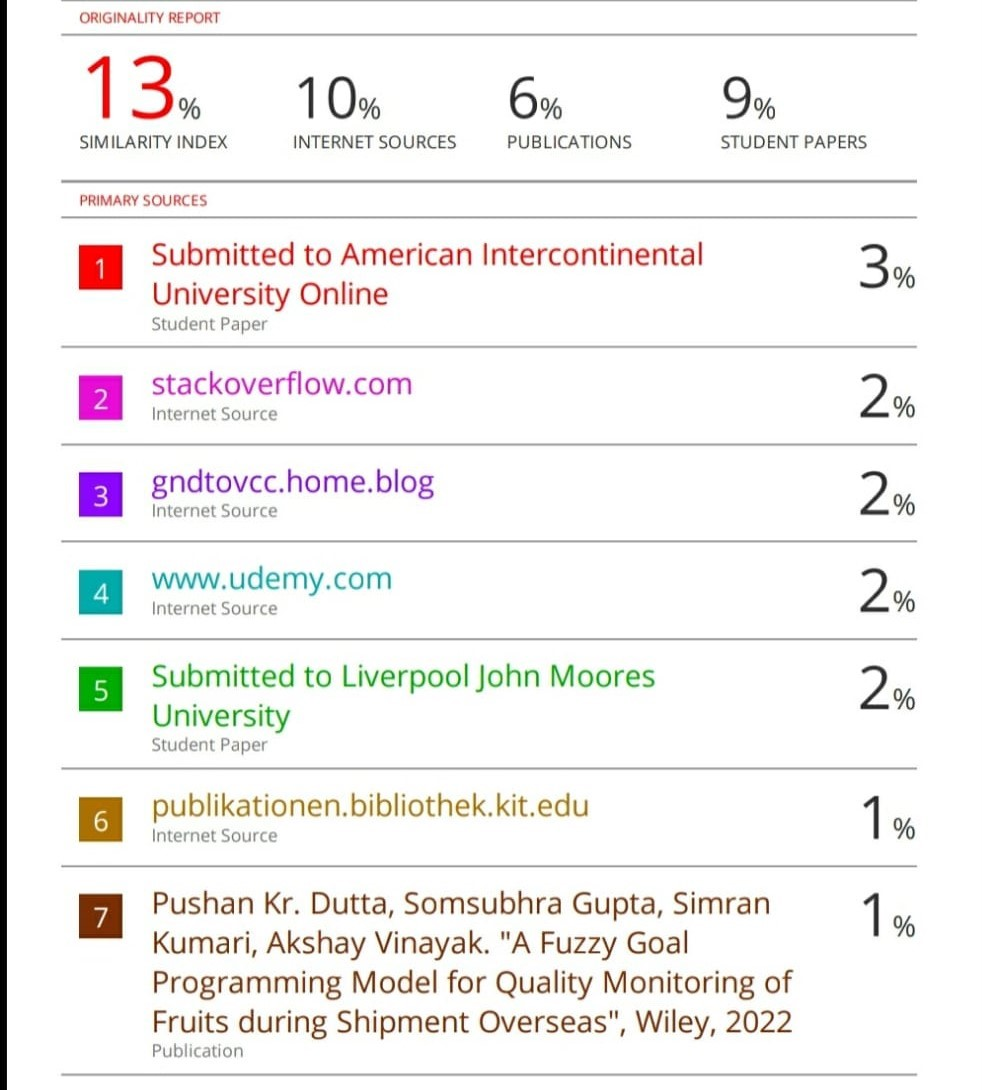
\includegraphics[width=14cm,height = 17cm,frame]{images/plag.jpeg}

\end{figure}


\newpage
\addcontentsline{toc}{chapter}{References}
\renewcommand\bibname{References}
\begin{thebibliography}{21}

\bibitem{paper1}Adela Has,Marijana Zeki´c-Suˇsac Machine learning based system for managing energy efficiency of public sector as an approach towards smart cities.\\

\bibitem{paper2}A Santollamazza, V Introna Anamoly Detection in Energy Consumption for Compressed Air Generation systems: an approach based on artificial neural networks.\\

\bibitem{paper3}Jianli Pan, Raj Jain, Subharthi Paul, Tam Vu, Abusayeed Saifullah An Internet of Things Framework for Smart Energy in Buildings: Designs, Prototype, and Experiments.
\bibitem{paper4}Qing Yang, Hao Wang Privacy-Preserving Transactive Energy Management
for IoT-aided Smart Homes via Blockchain.

\bibitem{paper5}Hyunjeong Lee, Sangkeun Yoo, Yong-Woon Kim An Energy Management Framework for Smart Factory based on Context-awareness.\\

\bibitem{paper6}Amam Hossain Bagdadee A Brief Review of the IoT-Based Energy Management System in the Smart Industry.

\bibitem{paper7}Arturs Purvins , Angelo L Abbate Automated energy management in distributed electricity systems: An EEPOS approach.

\bibitem{paper8}Syed Saqib Ali and Bong Jun Choi State-of-the-Art Artificial Intelligence Techniques for Distributed Smart Grids.

\bibitem{paper9}Naser Hossein Motlagh, Mahsa Mohammadrezaei and Julian Hunt Internet of Things (IoT) and the Energy Sector.

\bibitem{paper10}Mark Ditsworth, Manish Niraula Machine Learning based Energy Management System for grid disaster
mitigation
\end{thebibliography}


\end{document}